\section{Segmentierung}
\writtenby{\dcauthornameewie}%
Die Segmentierung findet Anwendung bei der Klassifizierung von Bildelementen.
Dabei wird jedes Pixel anhand eines Kriteriums einer Klasse zugeordnet.
Ein simples Verfahren ist dabei die Verwendung eines Schwellwertes, das sogenannte \emph{Thresholding}.
%
  \[ C_I^{(n)}(x,y) = \begin{cases}[c@{\quad}r@{}c@{}l@{}]
       0      &              & \;I(x,y) & \;<    t_1     \\
       1      & t_1     \leq & \;I(x,y) & \;<    t_2     \\
       \vdots &              &   \vdots &                \\
       n-2    & t_{n-2} \leq & \;I(x,y) & \;<    t_{n-1} \\
       n-1    &              & \;I(x,y) & \;\geq t_{n-1}
     \end{cases} \]
%
Eine der häufigsten Anwendungen ist die Einteilung eines Bildes in zwei Klassen, z.B. Vorder- und Hintergrund.
%
  \[ C_I^{(2)}(x,y) = \begin{cases}
       0 & I(x,y) <    t \\
       1 & I(x,y) \geq t
     \end{cases} \]
%
Die Berechnung des Schwellwerts $t$ ist dabei entscheidend für die Qualität der Segmentierung, d.h. dass Bildelemente korrekt klassifiziert werden.

\subsection*{Schwellwertbestimmung}
Da die Wahl des Schwellwertes ausschlaggebend für die Genauigkeit der Klassifizierung ist, existieren diverse Algorithmen.
Diese machen sich zum Teil bestimmte Eigenschaften eines Bildes zu nutze und sind daher nur für eine bestimmte Klasse von Bildern geeignet, nämlich solche die jene Eigenschaften erfüllen.

\subsubsection*{Mittelwert}
Nutzt den Mittelwert der Helligkeit aller Bildpunkte als Schwellwert.
Der ermittelte Schwellwert ist sinnvoll, wenn sich Bildelemente durch ihre Helligkeits bereits deutlich vom Hintergrund abheben.
Im Allgemeinen ist der Mittelwert jedoch nicht optimal da dieser die Helligkeitsverteilung der Bildpunkte nicht berücksichtigt.
  \[ t = \frac{1}{N} \sum_{x,y} I(x,y), \quad N = \sum_{x,y} 1 \]

\subsubsection*{Iteratives Verfahren}
\ldots
\todo[author=\dcauthornameewie]{Iteratives Verfahren}

\subsubsection*{Otsu's Methode}
\surname{Otsu}'s Methode \cite{otsu1979} ist ein histogrammbasiertes Verfahren, dass eine bimodale Helligkeitsverteilung\footnote{Eine bimodale Helligkeitsverteilung besitzt zwei Maxima die den Helligkeitswerten des Hintergrund bzw. Vordergrund entsprechen. Der optimale Schwellwert liegt im Tal zwischen den Maxima.} voraussetzt.
Der Algorithmus sucht den Schwellwert, der die Varianz innheralb der beiden Klassen minimiert.

\subsubsection*{Balanced Histogram Thresholding}
Das Balanced Histogram Thresholding \cite{DBLP:conf/biostec/AnjosS08} erwartet, wie \surname{Otsu}'s Methode, eine bimodale Helligkeitsverteilung.
Das Verfahren ermittelt den Schwellwert derart, dass dieser das Histogramm in zwei gleich "`schwere"' Hälften teilt.
Als Maß für das Gewicht einer Hälfte dient die Summe der absoluten Häufigkeiten aller Klassen der betrachteten Hälfte.
Von der schwereren Häfte wird solange die äußere Klasse entfernt bis nur noch eine Klasse übrig ist, welche dem gesuchten Schwellwert entspricht.

\subsection*{Anwendungsbereich des Thresholding}
Die Berechnung und Anwendung eines Schwellwertes ist nicht auf das Gesamtbild beschränkt, sondern kann granularer gestaltet sein um z.B. ungleichmäßige Beleuchtung zu behandeln.

\subsubsection*{Statisches Thresholding}
Der Schwellwert wird für das gesamte Bild einmalig berechnet und auf alle Bildpunkte angewandt.
Die Verwendung eines einzelnen Schwellwertes für das gesamte Bild funkioniert nur sofern das Bild gleichmäßig belichtet ist \cite[Kap.~4.3]{davies2012}.
Ansonsten kann es vorkommen, zu dunkle Bildteile, aufgrund zu geringer Belichtung, als Hintergrund zu klassifizieren da diese unterhalb des Schwellwertes liegen.

\subsubsection*{Dynamisches Thresholding}
Adaptives Thresholding ermöglicht es Bilder mit ungleichmäßiger Beleuchtung besser zu Segmentieren.
Eine Möglichkeit ist es das Bild in Rechtecke zu unterteilen und auf jede Region das statische Thresholding anzuwenden \cite[Kap.~4.4,~S.~88--89]{davies2012}.
Dabei kann es an den Regionsgrenzen zu unterschiedlichen Klassifikationen kommen.
Ein besseres Verfahren stellt die Berechnung eines individuellen Schwellwertes für jeden Bildpunkt, unter Betrachtung seiner Umgebung, dar \cite[Kap.~4.4.2]{davies2012}.

\begin{figure}[H]
  \label{fig:segmentation}
  \centering
  \begin{subfigure}{0.49\linewidth}
    \centering
    
\includegraphics[width=\linewidth]{img/basics/segmentation/original}
    \caption{Original (526$\times$176)}
  \end{subfigure}
  \begin{subfigure}{0.49\linewidth}
    \centering
    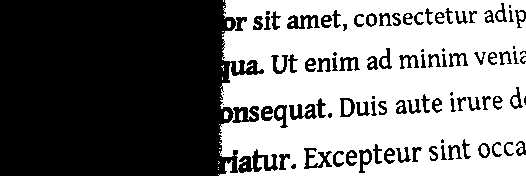
\includegraphics[width=\linewidth]{img/basics/segmentation/global}
    \caption{statisch}
  \end{subfigure}
  \begin{subfigure}{0.49\linewidth}
    \centering
    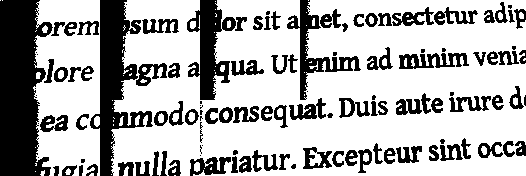
\includegraphics[width=\linewidth]{img/basics/segmentation/local}
    \caption{dynamisc, Einteilung in 100$\times$100 Pixel große Regionen}
  \end{subfigure}
  \begin{subfigure}{0.49\linewidth}
    \centering
    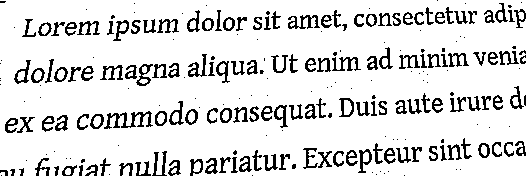
\includegraphics[width=\linewidth]{img/basics/segmentation/dynamic}
    \caption{dynamisc, Betrachtung einer 3$\times$3 Nachbarschaft}
  \end{subfigure}
  \caption[Vergleich von Thresholding Varianten]{Vergleich von Thresholding Varianten für Text bei ungleichmäßiger Belichtung. Als Schwellwert dient jeweils der oben beschriebene Mittelwert.}
\end{figure}
